% Source of the four diagrams in Recurring tricks.
% Compile each with: pdflatex "\def\SSACase{1}% Source of the four diagrams in Recurring tricks.
% Compile each with: pdflatex "\def\SSACase{1}% Source of the four diagrams in Recurring tricks.
% Compile each with: pdflatex "\def\SSACase{1}% Source of the four diagrams in Recurring tricks.
% Compile each with: pdflatex "\def\SSACase{1}\input{ssa-cases.tex}"
% SSACase takes values 1, 2, 3, 4. Coordinates are illustrative only;
% the displayed labels and conditions are general, not numerical examples.
\documentclass[tikz,border=8pt]{standalone}
\usetikzlibrary{calc,arrows.meta}
\providecommand\SSACase{1}
\begin{document}
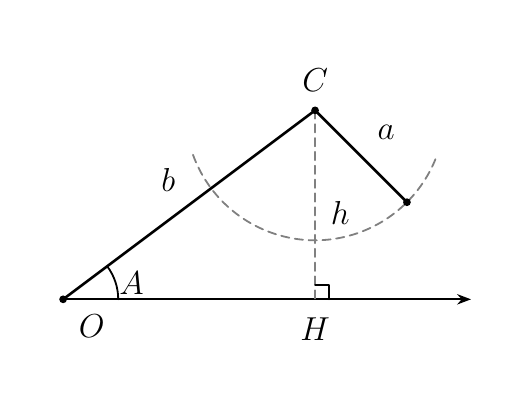
\begin{tikzpicture}[x=1cm,y=1cm,line cap=round,line join=round,
  font=\fontsize{13}{16}\selectfont,
  side/.style={line width=.95pt},
  guide/.style={gray,densely dashed,line width=.65pt},
  lab/.style={inner sep=1.5pt}]
  \coordinate (O) at (0,0);
  \coordinate (C) at (3.2,2.4);
  \coordinate (H) at (3.2,0);
  \ifcase\SSACase\or
    \def\rad{1.65}\def\edge{5.3}\def\leftedge{-.45}
  \or
    \def\rad{2.4}\def\edge{5.8}\def\leftedge{-.45}
  \or
    \def\rad{3}\def\edge{6.35}\def\leftedge{-.45}
  \or
    \def\rad{4.6}\def\edge{7.9}\def\leftedge{-1.35}
  \fi
  \path[use as bounding box] (\leftedge,-.85) rectangle (\edge,3.45);
  % The lower circular arc is the part relevant to intersections with the ray.
  \begin{scope}
    \clip (\leftedge,-.62) rectangle (\edge,3.4);
    \draw[guide] ($(C)+(200:\rad)$) arc[start angle=200,end angle=340,radius=\rad];
  \end{scope}
  \ifnum\SSACase=4
    \draw[guide] (-1.15,0)--(O);
  \fi
  \draw[-{Stealth[length=5pt]},line width=.65pt] (O)--(\edge-.12,0);
  \draw[side] (O)--node[lab,above left=3pt] {$b$}(C);
  \draw[line width=.65pt] (.7,0) arc[start angle=0,end angle=36.86989765,radius=.7];
  \node[lab] at (.87,.20) {$A$};
  \ifnum\SSACase=2
    \draw[side] (C)--(H);
    \node[lab,left=5pt] at (3.2,1.35) {$a$};
    \node[lab,right=5pt] at (3.2,1.35) {$h$};
  \else
    \draw[guide] (C)--(H);
    \node[lab,right=4pt] at (3.2,1.1) {$h$};
  \fi
  \draw[line width=.55pt] (3.2,.18)--(3.38,.18)--(3.38,0);
  \fill (O) circle (1.4pt);\fill (C) circle (1.4pt);
  \node[lab,above=5pt] at (C) {$C$};
  \node[lab,below right=4pt] at (O) {$O$};
  \ifnum\SSACase=1
    \coordinate (D) at ($(C)+(-45:\rad)$);
    \draw[side] (C)--node[lab,above right=4pt] {$a$}(D);
    \fill (D) circle (1.4pt);
    \node[lab,below=5pt] at (H) {$H$};
  \fi
  \ifnum\SSACase=2
    \fill (H) circle (1.4pt);
    \node[lab,below=5pt] at (H) {$B=H$};
  \fi
  \ifnum\SSACase=3
    \coordinate (B1) at (1.4,0);\coordinate (B2) at (5,0);
    \draw[side,dashed] (C)--node[lab,left=6pt,pos=.65] {$a$}(B1);
    \draw[side] (C)--node[lab,above right=4pt,pos=.52] {$a$}(B2);
    \fill (B1) circle (1.4pt);\fill (B2) circle (1.4pt);
    \node[lab,below=5pt] at (B1) {$B_1$};
    \node[lab,below right=5pt] at (B2) {$B_2$};
    \node[lab,below=5pt] at (H) {$H$};
  \fi
  \ifnum\SSACase=4
    \pgfmathsetmacro\dx{sqrt(\rad*\rad-2.4*2.4)}
    \coordinate (B) at (3.2+\dx,0);
    \coordinate (X) at (3.2-\dx,0);
    \draw[side] (C)--node[lab,above right=4pt,pos=.48] {$a$}(B);
    \draw[gray,line width=.7pt] ($(X)+(-.06,-.06)$)--($(X)+(.06,.06)$)
      ($(X)+(-.06,.06)$)--($(X)+(.06,-.06)$);
    \fill (B) circle (1.4pt);
    \node[lab,below right=5pt] at (B) {$B$};
    \node[lab,below=5pt] at (H) {$H$};
    \node[lab,below left=5pt] at (X) {$X$};
  \fi
\end{tikzpicture}
\end{document}
"
% SSACase takes values 1, 2, 3, 4. Coordinates are illustrative only;
% the displayed labels and conditions are general, not numerical examples.
\documentclass[tikz,border=8pt]{standalone}
\usetikzlibrary{calc,arrows.meta}
\providecommand\SSACase{1}
\begin{document}
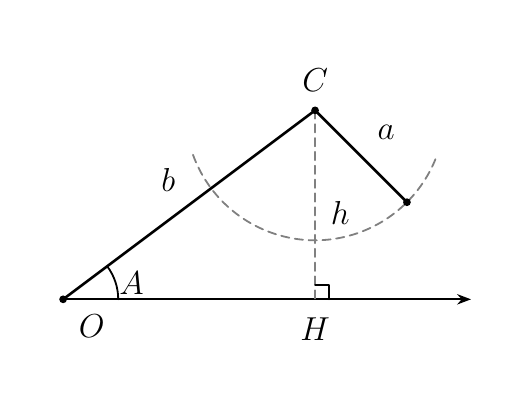
\begin{tikzpicture}[x=1cm,y=1cm,line cap=round,line join=round,
  font=\fontsize{13}{16}\selectfont,
  side/.style={line width=.95pt},
  guide/.style={gray,densely dashed,line width=.65pt},
  lab/.style={inner sep=1.5pt}]
  \coordinate (O) at (0,0);
  \coordinate (C) at (3.2,2.4);
  \coordinate (H) at (3.2,0);
  \ifcase\SSACase\or
    \def\rad{1.65}\def\edge{5.3}\def\leftedge{-.45}
  \or
    \def\rad{2.4}\def\edge{5.8}\def\leftedge{-.45}
  \or
    \def\rad{3}\def\edge{6.35}\def\leftedge{-.45}
  \or
    \def\rad{4.6}\def\edge{7.9}\def\leftedge{-1.35}
  \fi
  \path[use as bounding box] (\leftedge,-.85) rectangle (\edge,3.45);
  % The lower circular arc is the part relevant to intersections with the ray.
  \begin{scope}
    \clip (\leftedge,-.62) rectangle (\edge,3.4);
    \draw[guide] ($(C)+(200:\rad)$) arc[start angle=200,end angle=340,radius=\rad];
  \end{scope}
  \ifnum\SSACase=4
    \draw[guide] (-1.15,0)--(O);
  \fi
  \draw[-{Stealth[length=5pt]},line width=.65pt] (O)--(\edge-.12,0);
  \draw[side] (O)--node[lab,above left=3pt] {$b$}(C);
  \draw[line width=.65pt] (.7,0) arc[start angle=0,end angle=36.86989765,radius=.7];
  \node[lab] at (.87,.20) {$A$};
  \ifnum\SSACase=2
    \draw[side] (C)--(H);
    \node[lab,left=5pt] at (3.2,1.35) {$a$};
    \node[lab,right=5pt] at (3.2,1.35) {$h$};
  \else
    \draw[guide] (C)--(H);
    \node[lab,right=4pt] at (3.2,1.1) {$h$};
  \fi
  \draw[line width=.55pt] (3.2,.18)--(3.38,.18)--(3.38,0);
  \fill (O) circle (1.4pt);\fill (C) circle (1.4pt);
  \node[lab,above=5pt] at (C) {$C$};
  \node[lab,below right=4pt] at (O) {$O$};
  \ifnum\SSACase=1
    \coordinate (D) at ($(C)+(-45:\rad)$);
    \draw[side] (C)--node[lab,above right=4pt] {$a$}(D);
    \fill (D) circle (1.4pt);
    \node[lab,below=5pt] at (H) {$H$};
  \fi
  \ifnum\SSACase=2
    \fill (H) circle (1.4pt);
    \node[lab,below=5pt] at (H) {$B=H$};
  \fi
  \ifnum\SSACase=3
    \coordinate (B1) at (1.4,0);\coordinate (B2) at (5,0);
    \draw[side,dashed] (C)--node[lab,left=6pt,pos=.65] {$a$}(B1);
    \draw[side] (C)--node[lab,above right=4pt,pos=.52] {$a$}(B2);
    \fill (B1) circle (1.4pt);\fill (B2) circle (1.4pt);
    \node[lab,below=5pt] at (B1) {$B_1$};
    \node[lab,below right=5pt] at (B2) {$B_2$};
    \node[lab,below=5pt] at (H) {$H$};
  \fi
  \ifnum\SSACase=4
    \pgfmathsetmacro\dx{sqrt(\rad*\rad-2.4*2.4)}
    \coordinate (B) at (3.2+\dx,0);
    \coordinate (X) at (3.2-\dx,0);
    \draw[side] (C)--node[lab,above right=4pt,pos=.48] {$a$}(B);
    \draw[gray,line width=.7pt] ($(X)+(-.06,-.06)$)--($(X)+(.06,.06)$)
      ($(X)+(-.06,.06)$)--($(X)+(.06,-.06)$);
    \fill (B) circle (1.4pt);
    \node[lab,below right=5pt] at (B) {$B$};
    \node[lab,below=5pt] at (H) {$H$};
    \node[lab,below left=5pt] at (X) {$X$};
  \fi
\end{tikzpicture}
\end{document}
"
% SSACase takes values 1, 2, 3, 4. Coordinates are illustrative only;
% the displayed labels and conditions are general, not numerical examples.
\documentclass[tikz,border=8pt]{standalone}
\usetikzlibrary{calc,arrows.meta}
\providecommand\SSACase{1}
\begin{document}
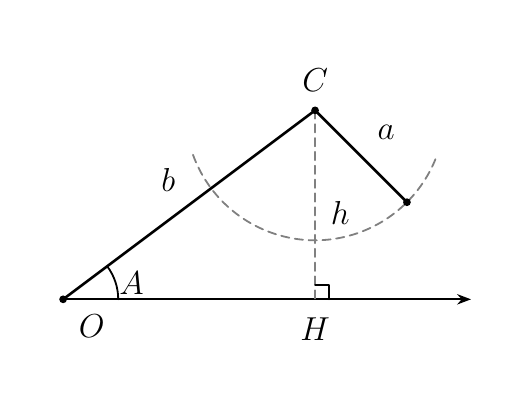
\begin{tikzpicture}[x=1cm,y=1cm,line cap=round,line join=round,
  font=\fontsize{13}{16}\selectfont,
  side/.style={line width=.95pt},
  guide/.style={gray,densely dashed,line width=.65pt},
  lab/.style={inner sep=1.5pt}]
  \coordinate (O) at (0,0);
  \coordinate (C) at (3.2,2.4);
  \coordinate (H) at (3.2,0);
  \ifcase\SSACase\or
    \def\rad{1.65}\def\edge{5.3}\def\leftedge{-.45}
  \or
    \def\rad{2.4}\def\edge{5.8}\def\leftedge{-.45}
  \or
    \def\rad{3}\def\edge{6.35}\def\leftedge{-.45}
  \or
    \def\rad{4.6}\def\edge{7.9}\def\leftedge{-1.35}
  \fi
  \path[use as bounding box] (\leftedge,-.85) rectangle (\edge,3.45);
  % The lower circular arc is the part relevant to intersections with the ray.
  \begin{scope}
    \clip (\leftedge,-.62) rectangle (\edge,3.4);
    \draw[guide] ($(C)+(200:\rad)$) arc[start angle=200,end angle=340,radius=\rad];
  \end{scope}
  \ifnum\SSACase=4
    \draw[guide] (-1.15,0)--(O);
  \fi
  \draw[-{Stealth[length=5pt]},line width=.65pt] (O)--(\edge-.12,0);
  \draw[side] (O)--node[lab,above left=3pt] {$b$}(C);
  \draw[line width=.65pt] (.7,0) arc[start angle=0,end angle=36.86989765,radius=.7];
  \node[lab] at (.87,.20) {$A$};
  \ifnum\SSACase=2
    \draw[side] (C)--(H);
    \node[lab,left=5pt] at (3.2,1.35) {$a$};
    \node[lab,right=5pt] at (3.2,1.35) {$h$};
  \else
    \draw[guide] (C)--(H);
    \node[lab,right=4pt] at (3.2,1.1) {$h$};
  \fi
  \draw[line width=.55pt] (3.2,.18)--(3.38,.18)--(3.38,0);
  \fill (O) circle (1.4pt);\fill (C) circle (1.4pt);
  \node[lab,above=5pt] at (C) {$C$};
  \node[lab,below right=4pt] at (O) {$O$};
  \ifnum\SSACase=1
    \coordinate (D) at ($(C)+(-45:\rad)$);
    \draw[side] (C)--node[lab,above right=4pt] {$a$}(D);
    \fill (D) circle (1.4pt);
    \node[lab,below=5pt] at (H) {$H$};
  \fi
  \ifnum\SSACase=2
    \fill (H) circle (1.4pt);
    \node[lab,below=5pt] at (H) {$B=H$};
  \fi
  \ifnum\SSACase=3
    \coordinate (B1) at (1.4,0);\coordinate (B2) at (5,0);
    \draw[side,dashed] (C)--node[lab,left=6pt,pos=.65] {$a$}(B1);
    \draw[side] (C)--node[lab,above right=4pt,pos=.52] {$a$}(B2);
    \fill (B1) circle (1.4pt);\fill (B2) circle (1.4pt);
    \node[lab,below=5pt] at (B1) {$B_1$};
    \node[lab,below right=5pt] at (B2) {$B_2$};
    \node[lab,below=5pt] at (H) {$H$};
  \fi
  \ifnum\SSACase=4
    \pgfmathsetmacro\dx{sqrt(\rad*\rad-2.4*2.4)}
    \coordinate (B) at (3.2+\dx,0);
    \coordinate (X) at (3.2-\dx,0);
    \draw[side] (C)--node[lab,above right=4pt,pos=.48] {$a$}(B);
    \draw[gray,line width=.7pt] ($(X)+(-.06,-.06)$)--($(X)+(.06,.06)$)
      ($(X)+(-.06,.06)$)--($(X)+(.06,-.06)$);
    \fill (B) circle (1.4pt);
    \node[lab,below right=5pt] at (B) {$B$};
    \node[lab,below=5pt] at (H) {$H$};
    \node[lab,below left=5pt] at (X) {$X$};
  \fi
\end{tikzpicture}
\end{document}
"
% SSACase takes values 1, 2, 3, 4. Coordinates are illustrative only;
% the displayed labels and conditions are general, not numerical examples.
\documentclass[tikz,border=8pt]{standalone}
\usetikzlibrary{calc,arrows.meta}
\providecommand\SSACase{1}
\begin{document}
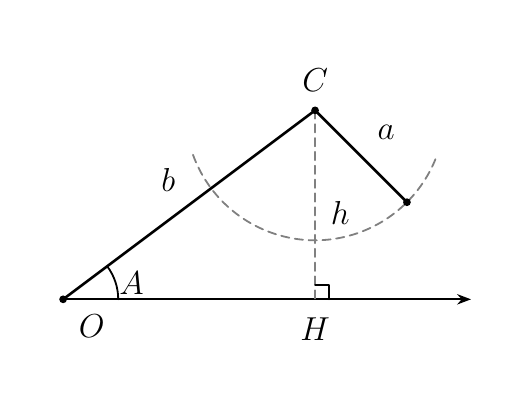
\begin{tikzpicture}[x=1cm,y=1cm,line cap=round,line join=round,
  font=\fontsize{13}{16}\selectfont,
  side/.style={line width=.95pt},
  guide/.style={gray,densely dashed,line width=.65pt},
  lab/.style={inner sep=1.5pt}]
  \coordinate (O) at (0,0);
  \coordinate (C) at (3.2,2.4);
  \coordinate (H) at (3.2,0);
  \ifcase\SSACase\or
    \def\rad{1.65}\def\edge{5.3}\def\leftedge{-.45}
  \or
    \def\rad{2.4}\def\edge{5.8}\def\leftedge{-.45}
  \or
    \def\rad{3}\def\edge{6.35}\def\leftedge{-.45}
  \or
    \def\rad{4.6}\def\edge{7.9}\def\leftedge{-1.35}
  \fi
  \path[use as bounding box] (\leftedge,-.85) rectangle (\edge,3.45);
  % The lower circular arc is the part relevant to intersections with the ray.
  \begin{scope}
    \clip (\leftedge,-.62) rectangle (\edge,3.4);
    \draw[guide] ($(C)+(200:\rad)$) arc[start angle=200,end angle=340,radius=\rad];
  \end{scope}
  \ifnum\SSACase=4
    \draw[guide] (-1.15,0)--(O);
  \fi
  \draw[-{Stealth[length=5pt]},line width=.65pt] (O)--(\edge-.12,0);
  \draw[side] (O)--node[lab,above left=3pt] {$b$}(C);
  \draw[line width=.65pt] (.7,0) arc[start angle=0,end angle=36.86989765,radius=.7];
  \node[lab] at (.87,.20) {$A$};
  \ifnum\SSACase=2
    \draw[side] (C)--(H);
    \node[lab,left=5pt] at (3.2,1.35) {$a$};
    \node[lab,right=5pt] at (3.2,1.35) {$h$};
  \else
    \draw[guide] (C)--(H);
    \node[lab,right=4pt] at (3.2,1.1) {$h$};
  \fi
  \draw[line width=.55pt] (3.2,.18)--(3.38,.18)--(3.38,0);
  \fill (O) circle (1.4pt);\fill (C) circle (1.4pt);
  \node[lab,above=5pt] at (C) {$C$};
  \node[lab,below right=4pt] at (O) {$O$};
  \ifnum\SSACase=1
    \coordinate (D) at ($(C)+(-45:\rad)$);
    \draw[side] (C)--node[lab,above right=4pt] {$a$}(D);
    \fill (D) circle (1.4pt);
    \node[lab,below=5pt] at (H) {$H$};
  \fi
  \ifnum\SSACase=2
    \fill (H) circle (1.4pt);
    \node[lab,below=5pt] at (H) {$B=H$};
  \fi
  \ifnum\SSACase=3
    \coordinate (B1) at (1.4,0);\coordinate (B2) at (5,0);
    \draw[side,dashed] (C)--node[lab,left=6pt,pos=.65] {$a$}(B1);
    \draw[side] (C)--node[lab,above right=4pt,pos=.52] {$a$}(B2);
    \fill (B1) circle (1.4pt);\fill (B2) circle (1.4pt);
    \node[lab,below=5pt] at (B1) {$B_1$};
    \node[lab,below right=5pt] at (B2) {$B_2$};
    \node[lab,below=5pt] at (H) {$H$};
  \fi
  \ifnum\SSACase=4
    \pgfmathsetmacro\dx{sqrt(\rad*\rad-2.4*2.4)}
    \coordinate (B) at (3.2+\dx,0);
    \coordinate (X) at (3.2-\dx,0);
    \draw[side] (C)--node[lab,above right=4pt,pos=.48] {$a$}(B);
    \draw[gray,line width=.7pt] ($(X)+(-.06,-.06)$)--($(X)+(.06,.06)$)
      ($(X)+(-.06,.06)$)--($(X)+(.06,-.06)$);
    \fill (B) circle (1.4pt);
    \node[lab,below right=5pt] at (B) {$B$};
    \node[lab,below=5pt] at (H) {$H$};
    \node[lab,below left=5pt] at (X) {$X$};
  \fi
\end{tikzpicture}
\end{document}
